\section{Background}\label[sec]{background}
\subsection{Potential, Limitations and Progress of the MAV}
Micro Areal Vehicles (MAVs) have great potential in contributing to indoor search-and-rescue missions. Their small size and weight
make them easy to transport and allows for rapid field deployment. Furthermore they are agile, allowing them to operate in 
complex environments and access hard-to-get-to places.

Limitations of current technologies, prohibiting the existence of fully autonomous MAVs, are examined in \cite{MAV_enabling}. They define the following
requirements for a fully autonomous MAV:
\begin{itemize}
  \item Inference: The ability to infer situational awareness from sensory measurements.
  \item Reasoning: The ability to define a mission based on abstract human-defined goals.
  \item Unsupervised learning: The ability to adapt and learn its own control strategies without human supervision.
\end{itemize}
Due to the constraints on the size of MAVs, the existence of fully autonomous MAVs is mainly dependent on the existence of 
small and efficient hardware components such as power supplies, sensors and processors allowing them to quickly process incoming data and convert this information into actions.
The authors of \cite{MAV_enabling} conclude that as of March 2017 no fully autonomous MAV system exist.

Although a fully autonomous MAV system is yet to be realized, the advancement in transistor density shown in \figref{trans_density}, and the continuously diminishing price of microprocessors continue to
allow for faster, and thus more complex, on-board computations. This allows for enhanced autonomous capabilities of the aircraft \cite{MAV_enabling}. Increased onboard computation power enables the aircraft to perform 
computations of increased complexity locally without the aid of other computation units or human interference, while conforming with real-time constraints.
\begin{figure}[H]
  \centering
  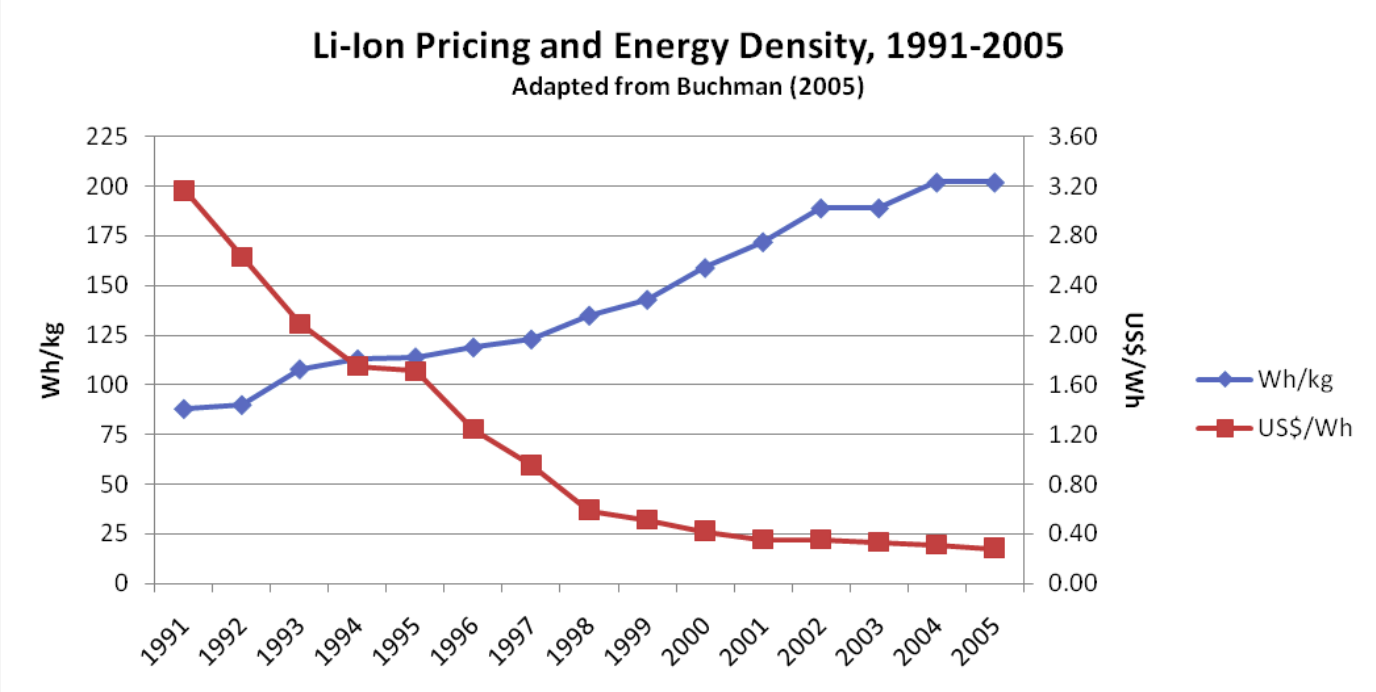
\includegraphics[width=.85\textwidth]{figs/lion-price.png}
  \caption{Evolution of energy density and cost of Lithium-ion batteries. Source: \cite{lion}.}
  \label[fig]{lion_price}
\end{figure}
\clearpage
\begin{figure}[h]
  \centering
  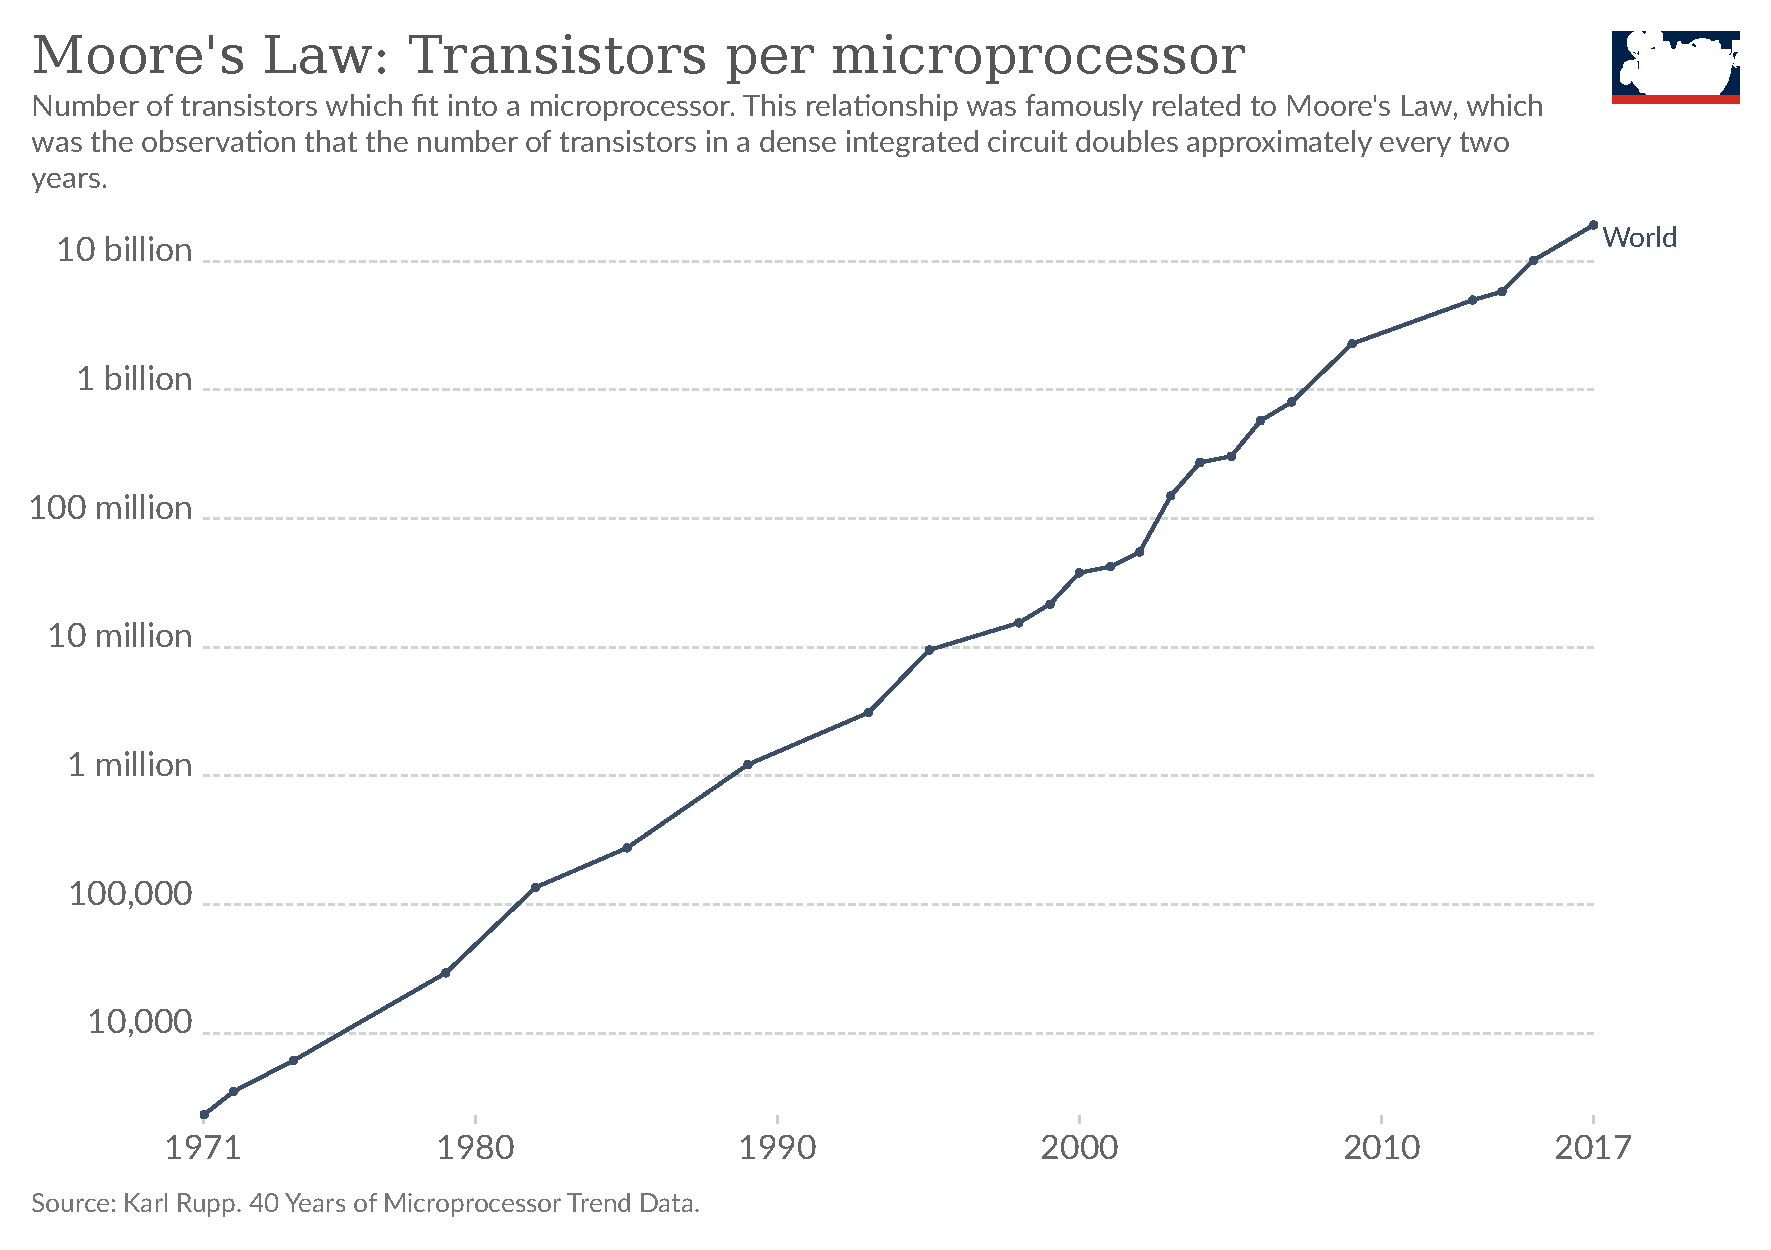
\includegraphics[width=.75\textwidth]{figs/transistors-per-microprocessor.pdf}
  \caption{Evolution of the number of transistors per microprocessor.}
  \label[fig]{trans_density}
\end{figure}

Most MAVs utilize electrical propulsion systems. This is due to the ability to miniaturize electrical propulsion systems for MAV applications with minimal loss of efficiency. Furthermore electrical propulsion systems have faster response time than combustion based systems \cite{MAV_enabling}. Energy is typically stored on
LiPo\footnote{Lithium-ion polymer} batteries. \figref{lion_price} shows how the energy density and price of Lithium-ion batteries have evolved over the last decades. As the energy density of Lithium-ion batteries already have and is projected to continue to increase \cite{lion_density}, this will allow 
for fitting more power consuming equipment on the MAVs, and increasing their endurance. Thus enabling MAVs to take on more complex and long lasting missions, resulting in increased autonomy.

Not only hardware components have made leaps over the last decades. The advancement in autonomy of MAV systems through the creation of efficient and lightweight software has been a field of great scientific interest.
The Robotics \& Perception Group at the University of Z\"urich have performed excessive research into the field of visual-inertial based real-time navigation and mapping
by MAVs in GNSS denied environments \cite{svo2, svo1}. The goal of which is enabling MAVs to localize themselves in and map unknown environments without external aid.

In \cite{svo2} a fast and robust visual-odometry algorithm (SVO) is presented. The method is faster than previously presented methods, and is therefore especially useful 
for MAV operations as it should be able to run on a onboard computer with limited processing power. It is concluded that the method is especially useful for state estimation onboard MAVs as the algorithm runs
at a high enough rate to provide accurate state estimates. Furthermore, the use of depth-filters yields an accurate map of the environment with few outliers.

In \cite{svo1} Scaramuzza et al. present a system for autonomous mapping of unknown indoor and outdoor environments performed by a single MAV using SVO. The MAV is supplied with 
a trajectory it is to follow, and using only on-board processing and sensing, follows said trajectory and provides at the same time a real-time map of the environment.

Developments such as those in \cite{svo2} and \cite{svo1} have increased the autonomous capabilities of MAVs, and as time passes more efficient software solutions will continue to do so.

\subsection{The Deployment Problem \& Blanket Coverage}
Multi-agent distributed control is the task of making a set of agents work together to fulfill some collective goal, and doing so 
with only local information. One such task is studied in this report, self-deployment: Make a swarm of robots "[...] deploy 
themselves in an environment without central coordination"\cite{BAYINDIR2016292}. A subcategory of the deployment problem is referred to 
in literature as the blanket coverage problem. In \cite{BAYINDIR2016292} the blanket coverage problem is defined as the task of finding a static 
configuration of agents such that a cost function is maximized over an area.

Cassandras and Zhong present in \cite{cassandras} a distributed method for a multi-agent blanket coverage.
They approach the blanket coverage problem using a probability based objective function. With their approach the 
goal of the set of agents is maximizing the joint detection probability of randomly occurring events in the environment. 
They also present an algorithm that preserves connectivity of the network of agents. They conclude that using their method, the swarm of agents reach a configuration corresponding to a 
local maxima of the joint detection probability function. Furthermore they find that when connectivity preservation is imposed, the swarm settles at a configuration in which the joint detection probability is
smaller than when connectivity of the network is not taken into account.

In \cite{sun2014escaping} Cassandras and Zhong "[...] address the problem of multiple local optima
commonly arising in optimization problems for multi-agent systems[...]". Utilizing the same probability based objective function as in \cite{cassandras}, boosting functions are applied to encourage agents to explore poorly
covered regions of the area and escape local optima. Three families of boosting functions are defined and tested through simulations. It is shown that the objective value post boosting is no worse than before.

Howard et.al. present in \cite{pot_field} another approach to the blanket coverage problem: virtual potential fields. It is assumed that 
agents are able to determine the range and bearing to both nearby agents and obstacles. Drawing inspiration from 
electrostatic fields, agents are seen on as point charges who exert repulsive forces on one another, causing them to spread. Furthermore
obstacles also exert forces on the agents so that agents do not collide with obstacles in the environment. They show through simulations
that the potential field approach can be used to deploy multi-agent networks for the means of blanket coverage, and conclude that area
coverage emerges from a combination of "[...] purely local rules"\cite{pot_field}.

\clearpage
\subsection{Multilateration}\label[ssec]{trilat}
Multilateration is the process of determining the positions of unknown points in space by measurements of distances from known points \cite{trilat_website}. In order
to perform this task in two-dimensional space, at least three known points are needed.

Given $n\geq 3$ beacons located at positions $\mathbf{x}_{a}\in\mathbb{R}^{2},\; 0\leq a<n$ where not all points
lie on a single line, the location 
of an entity, denoted by $\mathbf{y}\in\mathbb{R}^{2}$, can be determined as follows:
\begin{enumerate}
  \item The entity broadcasts signal and starts a timer at $t_{0}$.
  \item Beacons at $\mathbf{x}_{a},\; 0\leq a<n$ receive broadcasted signal and immediately responds with a packet containing $\mathbf{x}_{a}$.
  \item When receiving the packet from beacon at $\mathbf{x}_{a}$, the entity stores the time of reception in a variable $t_{1, a}$.
  \item When at least 3 beacons have responded, the entity calculates the distance
  from itself to beacon at $\mathbf{x}_{a}$: $d_{a} = \frac{1}{2}s(t_{1, a} - t_{0})$, where $s$ is the propagation speed of the signal. The factor $\frac{1}{2}$ is due to the signal traveling
  two times the distance between the entity and the beacon placed at $\mathbf{x}_{a}$ (the ping travels from the entity to the agent, and the packet
  sent by the agent travels back again).
  \item Based on the distances, $d_{a}$, and the positions of the beacons the entity can
  determine its position by calculating the point where circles centered at $\mathbf{x}_{a}$ with radii $d_{a}$ intersect.
\end{enumerate}
If sufficiently many beacons respond an ML (Maximum Likelihood) estimator of the position of the entity can be computed \cite{10.1145/381677.381693}.
Defining the error function:\begin{equation}
  e_{a}(\mathbf{y}) = s(t_{1, a} - t_{0, a}) - \norm{\mathbf{x}_{a} - \mathbf{y}} = d_{a} - \norm{\mathbf{x}_{a} - \mathbf{y}}
\end{equation}
An estimate of the position of the entity is obtained by solving:
\begin{equation}
  \hat{\mathbf{y}} = \argmin_{\mathbf{y}} \mathbf{E}^{T}\mathbf{E},\quad\mathbf{E} = \begin{bmatrix}
    e_{0}(\mathbf{y})\\
    \vdots\\
    e_{n-1}(\mathbf{y})
  \end{bmatrix}
\end{equation}
The position estimation error is affected by the measurement errors, by the geometry relating sensors and target, and by the estimation algorithm \cite{trilat_error}.
As the pings travel at large velocities (the speed of light) the resolution of the internal clock of the parties involved set a bound on the accuracy of the estimated position.
As was found in \cite{CRB_multilat}, multilateration of the unknown position of an entity is most accurate when the entity is placed nearby or within the convex hull of the beacons. Hence spreading
the beacons is desirable in order to obtain accurate position estimates.
\figref{trilat_example} shows how the position of an entity can be determined from the known positions of 3 agents.
\begin{figure}[H]
  \centering
  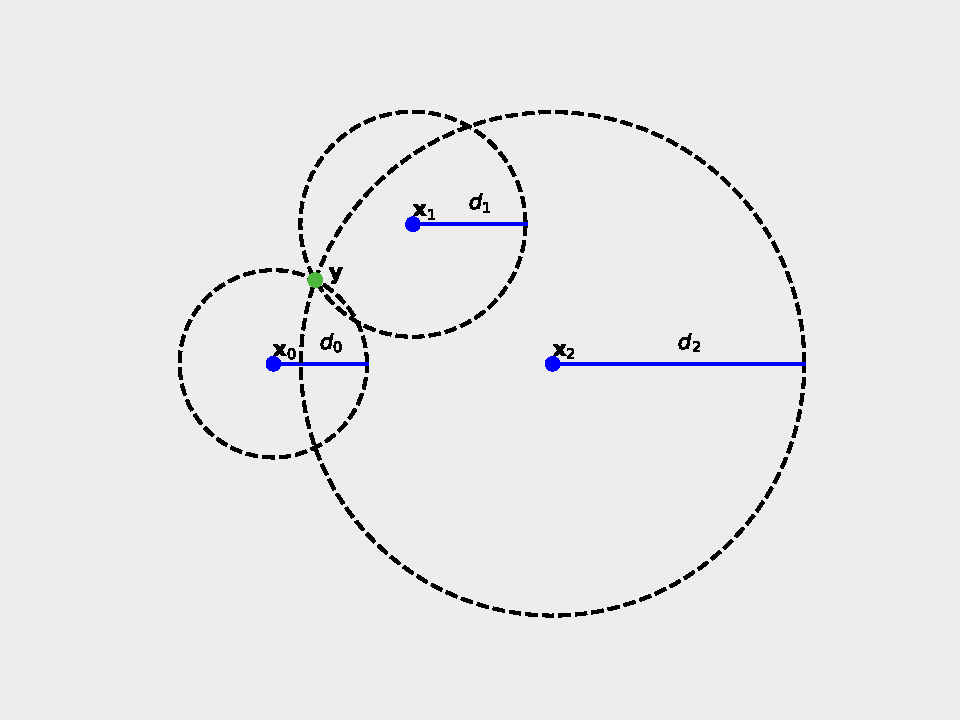
\includegraphics[width=.7\textwidth]{figs/trilateration_example.pdf}
  \caption{Position, $\mathbf{y}$, of entity determined by multilateration using known positions of $3$ beacons placed at $\mathbf{x}_{0}$, $\mathbf{x}_{1}$ and $\mathbf{x}_{2}$. The distances
  $d_{0}$, $d_{1}$ and $d_{2}$ are determined by sending pings between the entity at $\mathbf{y}$ and the beacons. The point $\mathbf{y}$ lies at the intersection of the circles placed at 
  $\mathbf{x}_{a}$ with radius $d_{a}$, $a = 0, 1, 2$.}
  \label[fig]{trilat_example}
\end{figure}